\begin{figure}[h!]
\centering
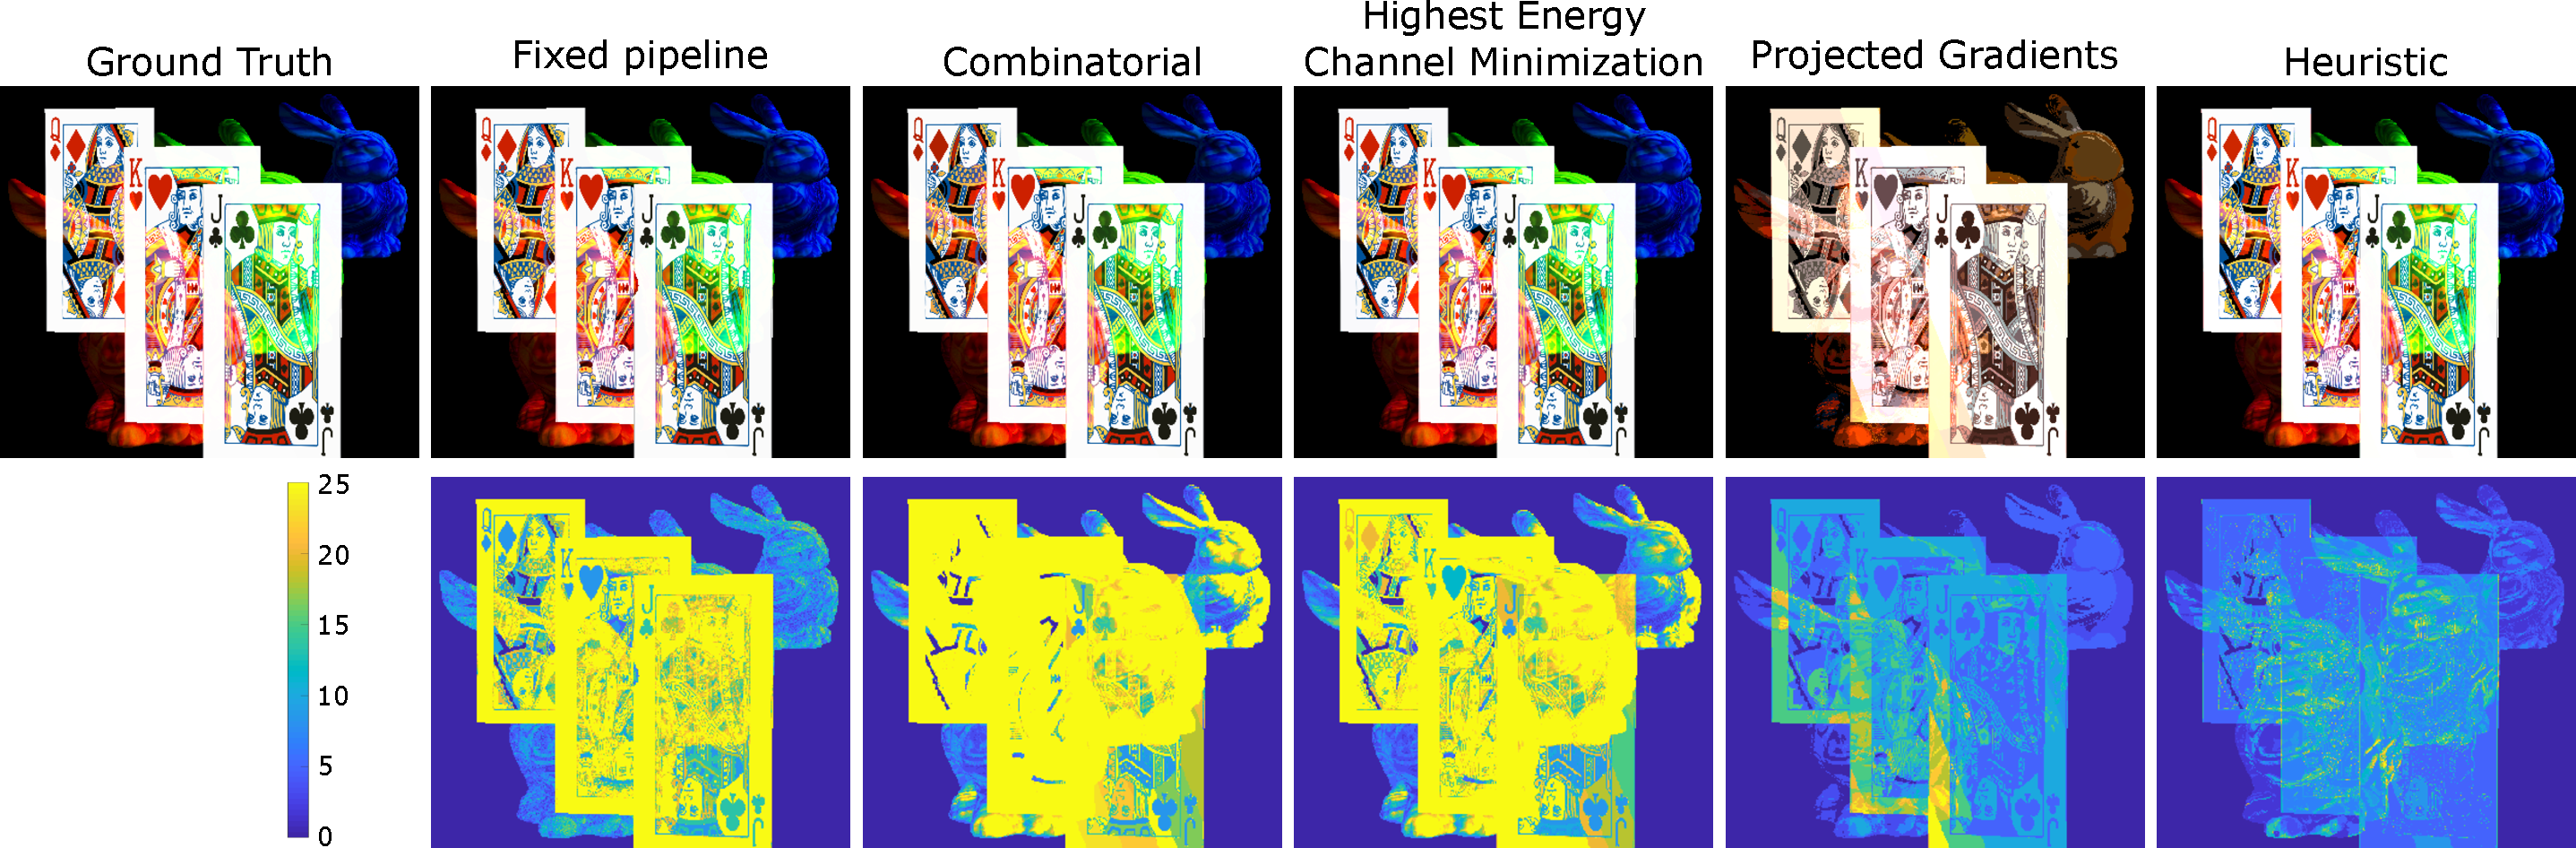
\includegraphics[width=0.99\columnwidth]{images/volumetric/acd_exp10/exp_pinhole}
\caption[Adaptive color decomposition: pinhole-camera reconstruction and number of binary voxels]{Simulation results. \emph{Top row:} Visual quality when assuming that the imaging camera is a pinhole camera. \emph{Bottom row:} Number of binary voxels for each color voxel.}
\label{fig:volumetric:acd:exp10:pinhole}
\end{figure}

